\chapter{Architettura di Sistema}
In questo capitolo viene descritta l'architettura \emph{hardware} del CPS in esame, in particolare, ne vengono evidenziati i \emph{Constituent System} (CS) e loro interfacce di comunicazione.
\section{Descrizione generale}
Lo scopo del sistema \`e quello di implementare un meccanismo di posizionamento basato su SFA.\\*
Tale algoritmo \`e schematizzabile come una \emph{black-box} (figura \ref{fig:sfa}) la quale prende in ingresso un certo insieme di misure, e fornisce in uscita una stima affidabile della posizione del treno lungo la traccia.\\*
\begin{figure}[h]
	\centering
	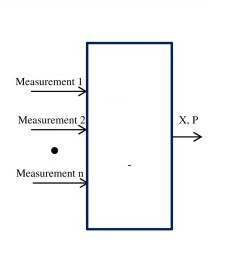
\includegraphics[scale=0.75]{img/sfaschema}
	\caption{Schema SFA}
	\label{fig:sfa}
\end{figure}
\clearpage
Questo algoritmo verr\`a eseguito su di un hardware installato a bordo treno, ed ha lo scopo di monitorare costantemente il moto dello stesso.\\*
Le grandezze fisiche che dovranno essere misurate e fornite a SFA sono:
\begin{itemize}
	\item Vettore accelerazione;
	\item Vettore velocit\`a angolare;
	\item Coordinate geografiche;
	\item Velocit\`a lineare (scalare).
\end{itemize}
SFA utilizzer\`a queste informazioni in combinazione con un'apposita digitalizzazione della traccia tramviaria su cui si trova il treno monitorato. Queste informazioni si suppongono note a priori ed accedibili tramite un \emph{database} caricato in memoria centrale.
\section{Constituent Systems}
Il sistema studiato si compone dei seguenti CS:
\begin{itemize}
	\item \emph{Sensor Set}, ossia un insieme di sensori atto a campionare le misure di interesse per il sistema. Il \emph{Sensor Set} \`e composto dai seguenti strumenti di misura:
	\begin{itemize}
		\item \emph{Inertial Measurement Unit} (IMU):\\*
		Sensore incaricato di misurare i vettori \texttt{accelerazione} ($\mathbf{a}$) e \texttt{velocit\`a angolare} ($\mathbf{v_{ang}}$) attraverso l'uso combinato di un accelerometro e un giroscopio. Le misure di IMU sono prese rispetto alla Terra e sono espresse in unit\`a stabilite dallo standard internazionale (SI):
		$$
		\mathbf{a}\;\left[\frac{m}{s^2}\right]\;\;\;\;\mathbf{v_{ang}}\;\left[ \frac{rad}{s} \right]
		$$
		Si tratta del sensore principale, infatti, date le caratteristiche intrinseche del particolare SFA utilizzato, il sistema potrebbe funzionare anche senza i rimanenti sensori; si apprezzerebbe tuttavia un calo delle performance in termini di errore commesso sulla stima della progressiva chilometrica della vettura.
		\begin{figure}[h]
			\centering
			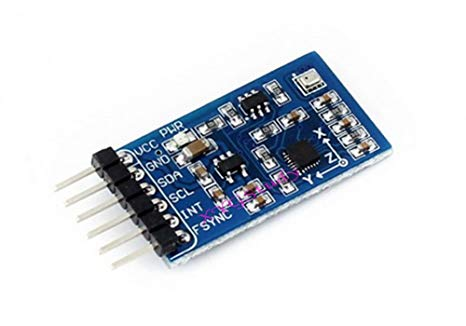
\includegraphics[width=\linewidth]{img/imu}
			\caption{\emph{Inertial Measurment Unit}}
			\label{fig:imu}
		\end{figure}
		\item Odometro:\\*
		Sistema composto da un emettitore e da un ricevitore radar, che fornisce al sistema le misure di velocit\`a lineare del treno attraverso il tempo impiegato da una ruota a compiere un giro completo.
		\item Ricevitore GPS:
		\\*Hardware in grado di ricevere informazioni sulle coordinate geografiche del treno. Fornisce le misure di posizione al sistema.\\*
Le misure di GPS sono riportate in formato standard come tripla di coordinate \texttt{(latitudine, longitudine, altitudine)}, rispettivamente espresse in gradi \texttt{N-S}, in gradi \texttt{E-O} e in \texttt{metri} sul livello del mare.\\*
	\end{itemize}
	\item Piattaforma di elaborazione dati. Consiste di una scheda \texttt{Nvidia TX-Jetson} su cui viene eseguito SFA.
	\item \emph{On Board Control Unit} (OBCU). Computer di bordo del treno. Esso non svolge alcun ruolo attivo nel sistema di posizionamento, tuttavia la progressiva chilometrica, stimata da SFA, dovr\'a essere trasmessa a OBCU al fine di poter utilizzare questa informazione all'interno del sistema di \emph{interlocking} della traccia.
\end{itemize}
	\section{Interfacce}
	Il CPS interagisce con l'ambiente attraverso le RUPI dei sensori. Queste interfacce acquisiscono, a diverse frequenze, i dati sul moto del treno che verranno elaborati dal resto del sistema di posizionamento.\\*
	Si distinguono due differenti RUMI alle quali avvengono le principali interazioni fra i CS:
	\begin{itemize}
		\item Tre bus dati, che collegano il \emph{Sensor Set} alla scheda \texttt{Nvidia TX-Jetson}. Su ciascuno di essi, \emph{Sensor Set} invia rispettivamente messaggi contenenti i dati campionati da IMU, Odometro e GPS.
		\item Interfaccia LTE. Essa permette di realizzare una \emph{rete wireless ad hoc} fra la scheda e OBCU.\\*
		All'interno di tale rete vengono instradati datagrammi \texttt{IP} contenenti le informazioni sulla progressiva chilometrica stimata da SFA, ed eventualmente messaggi di \emph{acknowledgment} di OBCU verso la scheda.
	\end{itemize}
	\begin{figure}[h]
		\centering
		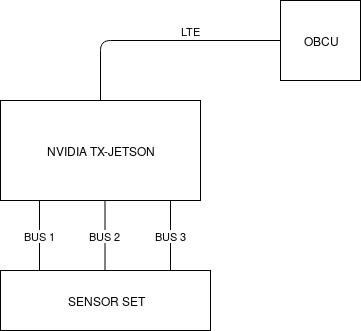
\includegraphics[width=0.7\linewidth]{img/TrainDiagram}
		\caption{Architettura hardware bordo treno}
		\label{fig:tdiagram}
	\end{figure}
	
